\RequirePackage{snapshot}
\documentclass[10pt,a4paper]{ULBreport}
\usepackage[utf8]{inputenc}
\sceau{Images/sceauULB.jpg}
\graphicspath{ {./Images/} }
\usepackage{multirow}
\usepackage{listings}
\usepackage{color} 
\usepackage{setspace} 
\usepackage{amsmath}

\usepackage{pdfpages}
\usepackage{biblatex}
\usepackage{floatrow}
\usepackage{subcaption} 
\usepackage{siunitx}
\usepackage[many]{tcolorbox}
\usepackage{multirow}
\usepackage{soul}
\usepackage[final]{pdfcomment}
\usepackage{listings}
\usepackage[dvipsnames]{xcolor}
\usepackage{fancyvrb}
\usepackage{hyperref}
\usepackage{xstring}
\usepackage{etoolbox}

% Colors


% BOXES FOR QUESTIONS

\newtcolorbox{questionBox}[2][]{
    fontupper=\bf,
    boxrule=1.5pt,
    colframe= black, % frame color
    fonttitle=\itshape,
    attach boxed title to top left={yshift=-0.3\baselineskip-0.4pt,xshift=2mm},
    title= #2,#1,
    enhanced,
    }

\newtcolorbox{bonusQuestionBox}[2][]{
    fontupper=\bf,
    boxrule=1.5pt,
    colframe= BlueViolet, % frame color
    colback=Periwinkle,
    coltitle=white,
    fonttitle=\itshape,
    attach boxed title to top left={yshift=-0.3\baselineskip-0.4pt,xshift=2mm},
    boxed title style={colback=Violet},
    title= #2,#1,
    enhanced,
    }





\begin{document} 


	\titleULB{
	title={Report Lab 2 \\ Tunnels and Encapsulation},
    studies={IRELE - MA1 Electrical Engineering},
    course ={ELEC-H417},
    author={\textit{Authors :} \\ Amaury ARICO \\ Alexis BOLLENGIER \\ Emmeran COLOT \\Sefa GÖNEN  },
    date={\textbf{Academic year :} \\ 2024 - 2025},
    teacher={\textit{Professor : } \\ Jean-Michel DRICOT \\\textit{Assistant : } \\ Navid LADNER },
    logo={Images/logo-polytech.jpg},
    manyAuthor
	}

\chapter{Mission 0 - No Tunnel Configuration}

\begin{figure}[H]
    \caption{Initial topology}
    \centering
    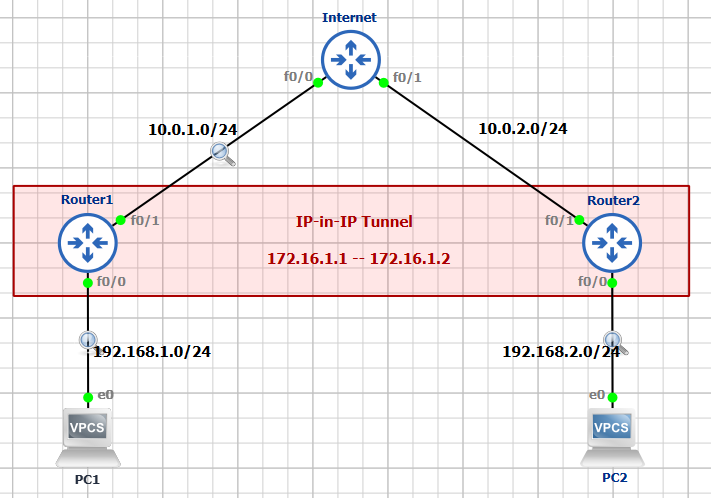
\includegraphics[width=0.7\textwidth]{Images/InitTopo.png}
    \label{initop}
\end{figure}

\section{Bonus question - Lost packet}

\begin{bonusQuestionBox}{Lost packet}
    Do you observe something special with the first (or two firsts) packet of the first ping command ? If yes, what is it and why ? (Wireshark could help)
\end{bonusQuestionBox}


% RESPONSE HERE

The figure \ref{fig:Images/Question_1_First_Pings_No_reply_2} shows the result of the ping command from \textbf{PC1} to \textbf{PC2} :

\begin{figure}[H]
    \caption{Ping command from PC1 (192.168.1.1) to PC2 (192.168.2.2)}
    \centering
    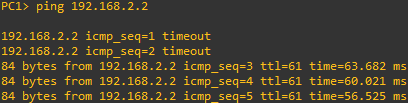
\includegraphics[width=0.7\textwidth]{Images/pingPC1PC2Commande.png}
    \label{fig:Images/Question_1_First_Pings_No_reply_2}
\end{figure}

We can observe that PC1 doesn't get a response (timeout) for the first 2 pings.
The reason is that \textbf{PC1} and \textbf{R1} didn't link their respective MAC addresses yet. It is also the case for \textbf{PC2} and \textbf{R2}.
\par
Indeed, by analysing the packet traffic on Wireshark, shown in the figures \ref{pingPC1PC2} and \ref{pingPC1PC22}, we can notice that the first ping request arrives at the last router R2 but this router doesn't have the MAC address of PC2 so that's why we get a timeout response for PC1 and an ARP request from R2 to PC2. \\
Concerning the second ping, the ping request arrives at PC2 but the ping reply doesn't go further than R1 because again, R1 didn't link its MAC address with PC1 (that's why we get a timeout response for the second ping and an ARP request from R1 to PC1).

\begin{figure}[H]
    \caption{Wireshark - Ping command from PC1 (192.168.1.1) to PC2 (192.168.2.2) - Listening to link between PC1 and R1}
    \centering
    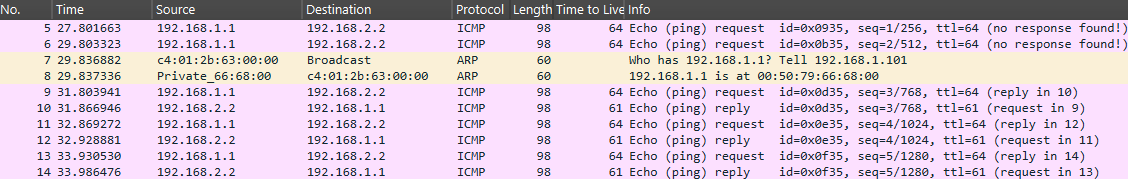
\includegraphics[width=\textwidth]{Images/pingPC1PC2.png}
    \label{pingPC1PC2}
\end{figure}

\begin{figure}[H]
    \caption{Wireshark - Ping command from PC1 (192.168.1.1) to PC2 (192.168.2.2) - Listening to link between PC2 and R2}
    \centering
    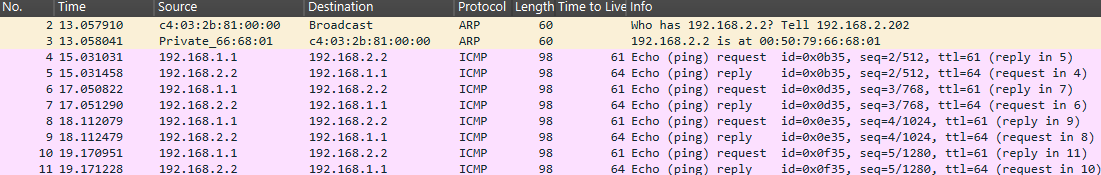
\includegraphics[width=\textwidth]{Images/pingPC1PC22.png}
    \label{pingPC1PC22}
\end{figure}


\chapter{Mission 1 - Site-to-Site Tunnel}

\section{Question - Netmask adaptation}

\begin{questionBox}{Netmask adaptation}
    What should be the netmask to achieve this and why ?
\end{questionBox}


% Response here

The trace command results (see figure \ref{tracePC1PC2} and \ref{tracePC2PC1}) gives us the following route :

\begin{center}
    \centering
    \textbf{PC1} $\leftrightarrow$ \textbf{R1} $\leftrightarrow$ \textbf{Internet}  $\leftrightarrow$ \textbf{R2}  $\leftrightarrow$ \textbf{PC2} 
\end{center}

\begin{figure}[H]
    \caption{Trace command result from PC1 (192.168.1.1) to PC2 (192.168.2.2)}
    \centering
    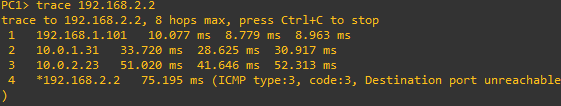
\includegraphics[width=0.8\textwidth]{Images/tracePC1PC2.png}
    \label{tracePC1PC2}
\end{figure}

\begin{figure}[H]
    \caption{Trace command result from PC2 (192.168.2.2) to PC1 (192.168.1.1)}
    \centering
    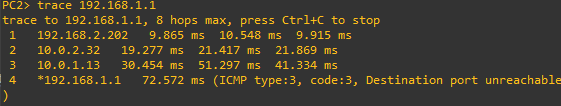
\includegraphics[width=0.8\textwidth]{Images/tracePC2PC1.png}
    \label{tracePC2PC1}
\end{figure}   

\section{Bonus question - One-way communication}

\begin{bonusQuestionBox}{One-way communication}
    What can you do to make a one way communication (i.e. ping PC1→PC2 works but not PC2→PC1) ?
\end{bonusQuestionBox}


% En gros PC1-> R1 rien de spécial, R1-> Internet, R1 encapsule le paquet (il met un nouveau IPv4 par dessus) et la nouvelle source devient le source du tunnel et la destination la destination du tunnel (pour UDP et ICMP !)
% But the ICMP response, we put the right tunnel IP !

% Question, que se passe-t-il si paquet ne passe pas par tunnel mais passe par R1 et internet (et part par exemple vers R3). Qu'est-ce qui se passe dans le cas d'un tunnel unidirectionnel ? Seulement encapsulation dans un seul sens ?

% Response here
The trace command results are shown in the figures \ref{tracePC1PC2tun} and \ref{tracePC2PC1tun}. For \textbf{PC1} $\rightarrow$ \textbf{PC2}, we have the route :

\begin{center}
    \centering
    \textbf{PC1} (192.168.1.1) $\rightarrow$ \textbf{R1} (192.168.1.101) $\rightarrow$ \textbf{R2} (172.16.1.2)  $\rightarrow$ \textbf{PC2} (192.168.2.2)
\end{center}

\begin{figure}[H]
    \caption{Trace command result from PC1 to PC2 -- bi-directional tunnel}
    \centering
    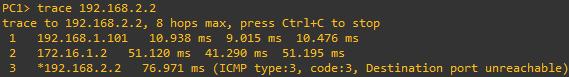
\includegraphics[width=0.8\textwidth]{Images/tracePC1PC2tun.png}
    \label{tracePC1PC2tun}
\end{figure}   

\begin{figure}[H]
    \caption{Trace command result from PC2 to PC1 -- bi-directional tunnel}
    \centering
    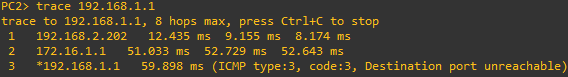
\includegraphics[width=0.8\textwidth]{Images/tracePC2PC1tun.png}
    \label{tracePC2PC1tun}
\end{figure}   

By using Wireshark and analysing the traffic for a trace command from PC1 to PC2 (see figures \ref{R1Int}, \ref{R2Int}, \ref{R2PC2}), we can observe the following : 

\begin{itemize}
    \item The \textbf{physical} route used by the packets is the same as before (before setting up the tunnel), see the figure \ref{tracePC1PC2} : \textbf{PC1} $\leftrightarrow$ \textbf{R1} $\leftrightarrow$ \textbf{Internet}  $\leftrightarrow$ \textbf{R2}  $\leftrightarrow$ \textbf{PC2}.
    \item The route seen by the packets' point of view is the route given by the trace command (figure \ref{tracePC1PC2tun}) : from their point of view, they don't go through the router Internet but rather \textbf{through the tunnel} we've configured.
    \item When packets from PC1 arrive at R1 (the same applies from PC2 to R2), a new IPv4 header is added on top of the original one. This process is called \textbf{encapsulation} and it is due to the tunnel we've set up in the router.
    \item When PC1 gets an ICMP reply from router R2, the IP source of this reply is 172.16.1.2 and not 10.0.2.23 (the IP destination of the new IPv4 header added in the UDP packet). Also we don't get an ICMP reply from the Internet router. That means the TTL in the UDP packet isn't decreased by this router but directly by R2.
\end{itemize}

From these observations, we can explain what is happening when we ping PC2 from PC1\footnote{We won't explain in detail here how the ping command works} : 


\begin{enumerate}
    \item PC1 creates UDP packets with an IPv4 header in which the source IP address is PC1's IP address (192.168.1.1) and destination IP address is PC2's IP address (192.168.2.2)
    \item The packet arrives at R1. At this stage, the router encapsulates the packet (see figure \ref{R1Int}) : the previous IPv4 header and payload become \textbf{the new payload} and a \textbf{new IPv4 header} is created with the source IP address being the tunnel source IP address (10.0.1.13) and the destination IP address being the tunnel destination IP address (10.0.2.23)
    \item The packet travels from R1 to R2 by going through the router Internet physically but from the packet points of view, it goes through the tunnel. That's why the TTL isn't decreased by the router Internet.
    \item The packet arrives at R2. This time, the router decapsulates the packet (see figure \ref{R2PC2}) : the new IPv4 header is removed and the previous IPv4 header in the payload is reestablished as the IP header.
    \item Packet arrives at PC2.
\end{enumerate}

\textbf{Remark} : we've configured a bi-directional tunnel

\begin{figure}[H]
    \caption{Wireshark screenshot - Trace command from PC1 to PC2 - Listening to link between R1 and Internet - in the red frame is the IPv4 header of the encapsulation and in the blue frame the payload of the encapsulation }
    \centering
    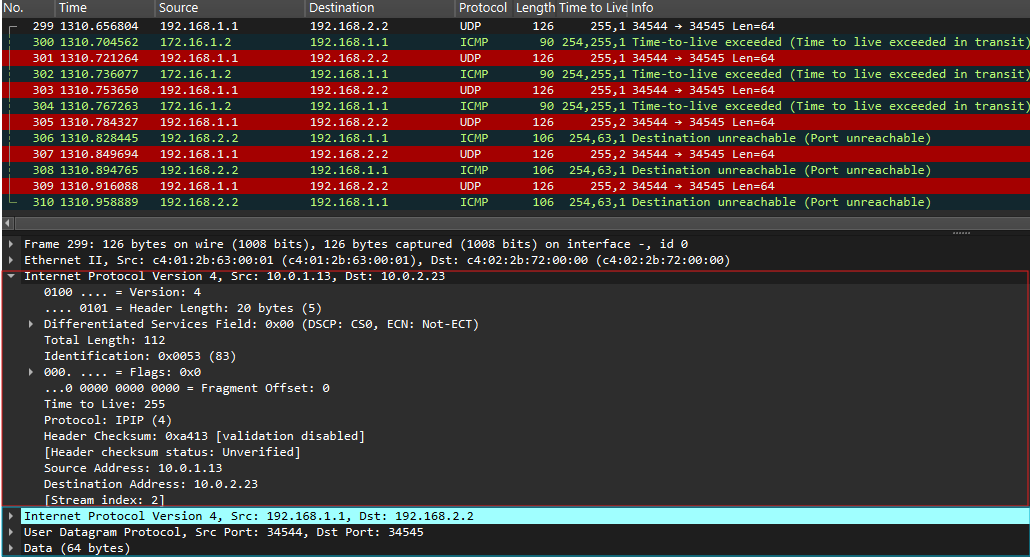
\includegraphics[width=\textwidth]{Images/traceWireR1Int.png}
    \label{R1Int}
\end{figure}

\begin{figure}[H]
    \caption{Wireshark screenshot - Trace command from PC1 to PC2 - Listening to link between R2 and Internet - in the red frame is the IPv4 header of the encapsulation and in the blue frame the payload of the encapsulation }
    \centering
    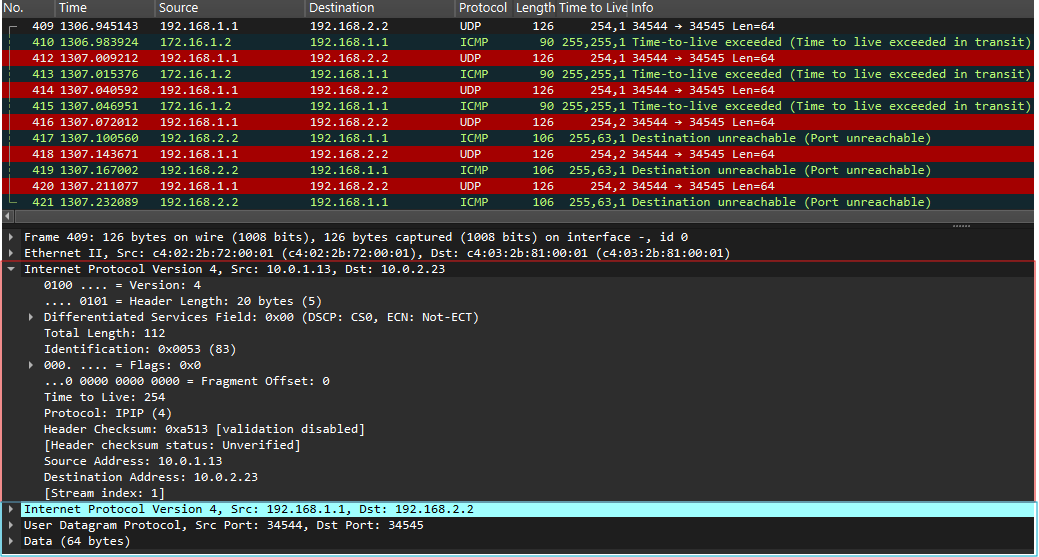
\includegraphics[width=\textwidth]{Images/traceWireR2Int.png}
    \label{R2Int}
\end{figure}

\begin{figure}[H]
    \caption{Wireshark screenshot - Trace command from PC1 to PC2 - Listening to link between R2 and PC2}
    \centering
    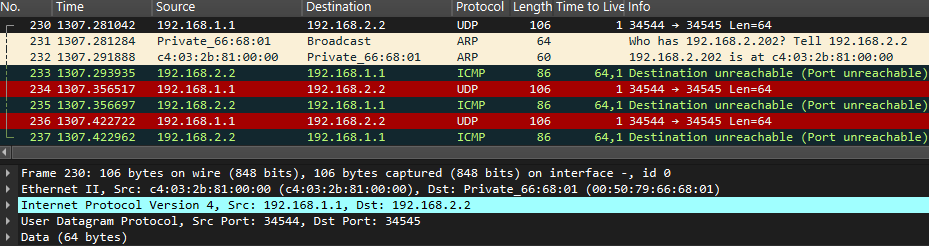
\includegraphics[width=\textwidth]{Images/traceWireR2PC2.png}
    \label{R2PC2}
\end{figure}

\chapter{Mission 2 - Deploy IPv6}

% frame.number<=251 && frame.number >=241&& _ws.col.protocol!=RIPv2 && _ws.col.protocol!=LOOP

\section{Question - IPv6 compatibility}

\begin{questionBox}{IPv6 compatibility}
    From PC1, ping Router1 and PC2 IPv4 and IPv6 addresses. What is working ? Why ?    
\end{questionBox}


Pinging the IPv4 addresses of \textbf{R1} (192.168.1.101) and of \textbf{PC2} (192.168.2.2) works fine (see figure \ref{ipv4}). This is not the case for IPv6 addresses :  only \textbf{R1} (FC00:1::101) replies to the ping as shown in the figure \ref{ipv6}.

\begin{itemize}
    \item \textbf{PC1} $\rightarrow$ \textbf{R1} : \textit{IPv4} and \textit{IPv6} works because PC1 and R1 are directly connected.
    \item \textbf{PC1} $\rightarrow$ \textbf{PC2} : \textit{IPv4} and \textit{IPv6} aren't compatible and the routers along the path know how to handle \textit{IPv4} addresses but not \textit{IPv6} addresses. The ping requests for IPv6 addresses don't go any further than R1 (FC00:1::101 replies "No route to destination").
\end{itemize}

\begin{figure}[H]
    \caption{Ping from PC1 (192.168.1.1) to R1 (192.168.1.101) and PC2 (192.168.2.2) IPv4 addresses}
    \centering
    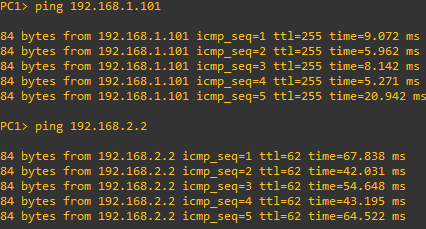
\includegraphics[width=0.7\textwidth]{Images/pingIPV4.png}
    \label{ipv4}
  \end{figure}

  \begin{figure}[H]
    \caption{Ping from PC1 (FC00:1::1) to R1 (FC00:1::101) and PC2 (FC00:2::2) IPv6 addresses}
    \centering
    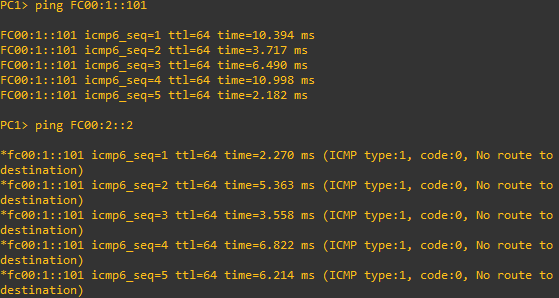
\includegraphics[width=0.7\textwidth]{Images/pingIPV6.png}
    \label{ipv6}
  \end{figure}


\section{Question - How does Traceroute reveal the path between devices ?}

\begin{questionBox}{ How does Traceroute reveal the path between devices ?}
    By analysing carefully your trace command using Wireshark (do not hesitate to capture all the three links), you should be able to understand how it works. Explain in details how the traceroute command works (and interesting observations you can make). What are the layer 3 protocols used and why ?
\end{questionBox}


\begin{itemize}
    \item The expanded form of the IPv6 address is FC00:0001:0000:0000:0000:0000:0000:0001/64.
    \item We need 128 bits to encode this address.
    \item \textbf{Subnet} : \textit{FC00:0001:0000:0000} (the last\footnote{We consider that the MSB is at the left} 64 bits)
    \item \textbf{Host} : \textit{0000:0000:0000:0001} (the first 64 bits)
    \item We can define $2^{64}$ IPv6 addresses for this specific subnet.
\end{itemize}

\chapter{Mission 3 - IPv6-in-IPv4 Tunnel}

\begin{figure}[H]
    \caption{New topology - 6in4 tunnel}
    \centering
    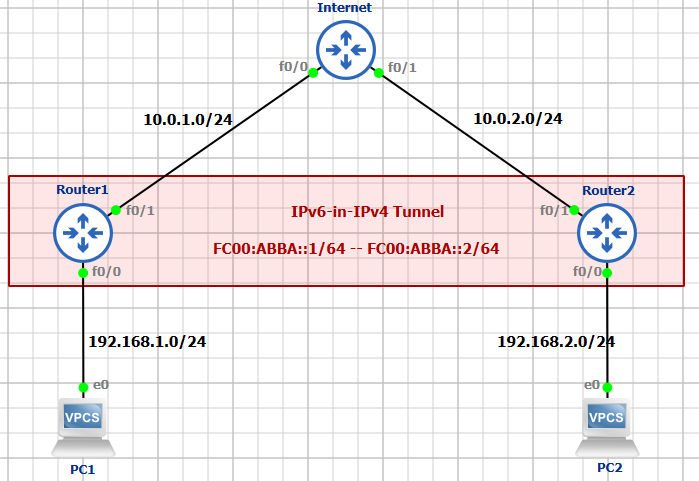
\includegraphics[width=0.7\textwidth]{Images/FinTopo.png}
    \label{Fintopo}
  \end{figure}

\section{Question - What is the route}

\begin{questionBox}{What is the route}
    What is the current route (IPs and devices) ? Did the route change (compared to mission 2: RIPv2) and why ?
\end{questionBox}




Considering the incompatibility of \textbf{IPv4}  and \textbf{IPv6}, the idea for the last mission is to use the tunnel to encapsulate the \textbf{IPv6} packet at the router \textbf{R1} by an \textbf{IPv4}  header and decapsulate the \textbf{IPv4}  header at the router \textbf{R2}, same thing as what we did for the \textit{mission 1}. \par
By proceeding in this way, we resolve the incompatibility between the networks and we are able to use \textbf{IPv6} addresses for the ping command.
The encapsulation is shown in a Wireshark screenshot (see figure ~\ref{fig:Images/Question_4_trace_PC2_Ipv6_Update_Wireshark_R1_internet_2}).

\begin{figure}[H]
  \caption{Wireshark screenshot - Trace command from PC1 (FC00:1::1) to PC2 (FC00:2::2) - Listening to link between R1 and Internet - in the red frame is the IPv4 header and in the blue frame the IPv6 payload}
  \centering
  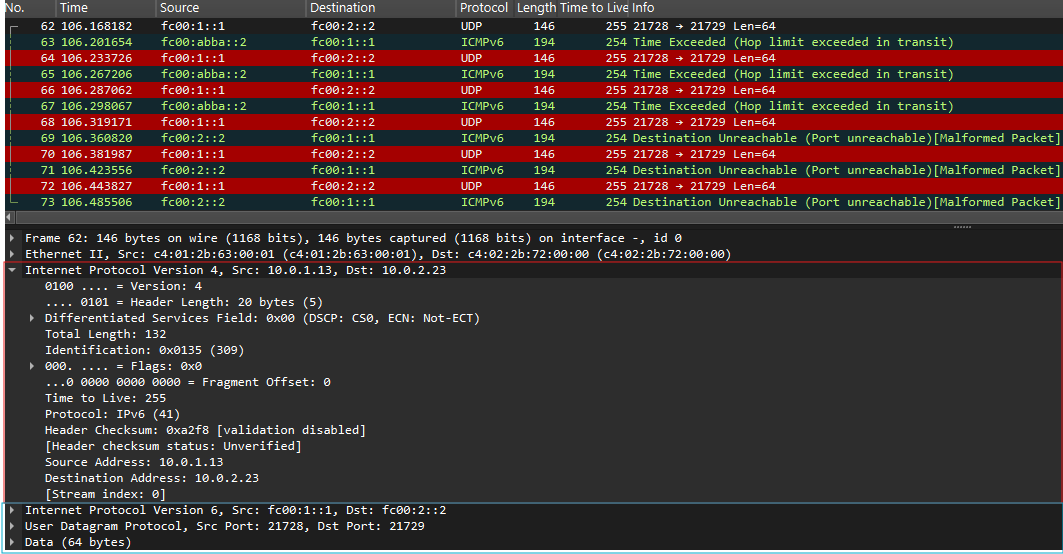
\includegraphics[width=\textwidth]{Images/traceIPV6.png}
  \label{fig:Images/Question_4_trace_PC2_Ipv6_Update_Wireshark_R1_internet_2}
\end{figure}

It should be mentionned that the tunnel mode has been reset from \textit{mode ipip} to \textit{mode ipv6ip}.
It implies that, from now on, only the \textbf{IPv6} packets are encapsulated by an \textbf{IPv4}  header at the tunnel. \\
The \textbf{IPv4} packets are no longer encapsulated as it was previously the case in the \textit{mission 1}.
This mode change can be noticed by comparing the trace command results for \textbf{IPv4} addresses and \textbf{IPv6} addresses, as shown in the figure ~\ref{fig:Images/Question_4_Difference_IPv4_IPv6}. \par
In fact, the route for the \textbf{IPv4} packet's point of view is the route passing by all the routers : \textbf{R1} $\leftrightarrow$ \textbf{Internet} $\leftrightarrow$ \textbf{R2}. \\
In the case of the \textbf{IPv6} packet perspective, the packet is going through the tunnel as it is encapsulated : \textbf{R1} $\leftrightarrow$ \textbf{R2}. \par
\textbf{Physically}, this is the same case as in the \textit{mission 1}, both \textbf{IPv4} and \textbf{IPv6} packets are taking the same route : \textbf{R1} $\leftrightarrow$ \textbf{Internet} $\leftrightarrow$ \textbf{R2}.

\begin{figure}[H]
  \caption{Trace route command from PC1 (192.168.1.1 / FC00:1::1) to PC2 (192.168.2.2 / FC00:2::2)}
  \centering
  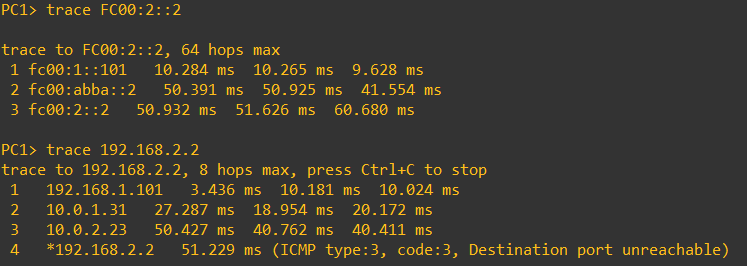
\includegraphics[width=0.8\textwidth]{Images/Question_4_Difference_IPv4_IPv6.png}
  \label{fig:Images/Question_4_Difference_IPv4_IPv6}
\end{figure}

\section{Question - What changes in the routing table after a network link failure ?}

\begin{questionBox}{What changes in the routing table after a network link failure ?}
    Display the routing table of your routers. What have changed ? How much time has it taken to change ? What could happen if you do a ping between PC1 and PC2 before the changes takes place ? What is the current route and its length ? Did the route change and why ?
\end{questionBox}


Many networks are still using the IPv4 (see figure \ref{ipv6adop}) and the problem is that it isn't compatible with IPv6. To be able to use IPv6 within older IPv4 networks, we resort to tunnels and encapsulation process to use IPv6 packets as IPv4 payloads (or the opposite depending on the route taken by the packet).

\begin{figure}[H]
    \caption{IPv6 Adoption - Percentage of users that acces Google over IPv6 over time - source \url{https://www.google.com/intl/en/ipv6/statistics.html} }
    \centering
    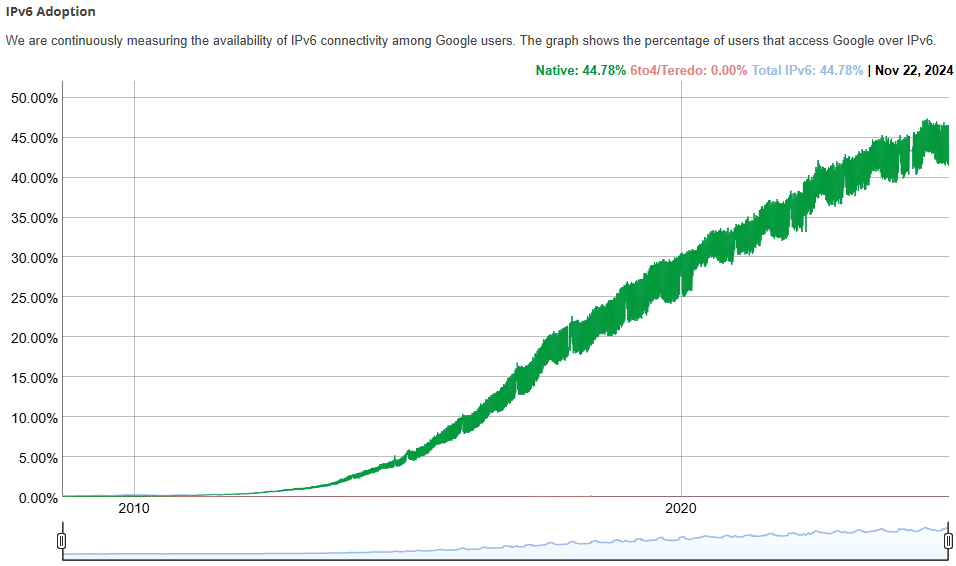
\includegraphics[width=0.9\textwidth]{Images/Ipv6adop.png}
    \label{ipv6adop}
  \end{figure}

\end{document}	

